% --- Program Section ---

\newprogram{Program 2}{Design a Sort class containing mergesort(arr: List[int]) -> List[int] and quicksort(arr:
List[int]) -> List[int] methods that accept an unsorted integer array and return the sorted
array.}

\subsection*{Code}
\begin{lstlisting}[language=Python]     % change the language attribute to C++ in case of C++ code.

from typing import List

class Sort:

    def merge_sort(self, arr: List[int]) -> List[int]:
        if len(arr) <= 1:
            return arr

        mid = len(arr) // 2

        left = self.merge_sort(arr[:mid])
        right = self.merge_sort(arr[mid:])

        return self.merge(left, right)

    def merge(self, left: List[int], right: List[int]) -> List[int]:
        result = []
        i = j = 0

        while i < len(left) and j < len(right):
            if left[i] <= right[j]:
                result.append(left[i])
                i += 1
            else:
                result.append(right[j])
                j += 1

        result.extend(left[i:])
        result.extend(right[j:])

        return result

    def quick_sort(self, arr: List[int]) -> List[int]:
        if len(arr) <= 1:
            return arr

        pivot = arr[len(arr) // 2]

        left = [x for x in arr if x < pivot]
        middle = [x for x in arr if x == pivot]
        right = [x for x in arr if x > pivot]

        return (
            self.quick_sort(left)
            + middle
            + self.quick_sort(right)
        )


# Example
s = Sort()

arr = [5, 2, 8, 1, 9, 3]

print("Merge Sort : " , s.merge_sort(arr))


print("Quick Sort : ", s.quick_sort(arr))

    
\end{lstlisting}

\subsection*{Output}
\begin{center}
    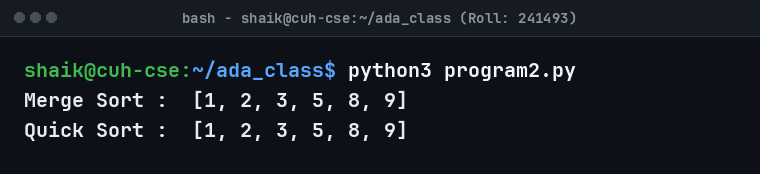
\includegraphics[width=0.88\textwidth]{Images/output_screenshot2.png}
\end{center}

\subsection*{GitHub Scan Code}
\begin{center}
    \begin{minipage}{0.3\textwidth}
        \centering
        % Generates a 2.5cm high QR code directly linking to the code file
        \qrcode[height=3.5cm]{https://github.com/gytdrop/ada_class/blob/main/program2.py} \\[0.2cm]
        \scriptsize\ttfamily Scan to view source code 
    \end{minipage}
\end{center}


% Add a horizontal line that indicates the END of the program.
\vspace{1cm}
\begin{center}
    \rule{1\textwidth}{1pt} % Clean, centered 1pt thick horizontal line
\end{center}